%\documentclass[draft,12pt]{jreport}
\documentclass[11pt,dvipdfmx]{ujreport}
\usepackage{siunitx}
\usepackage{amsmath}
\usepackage{sty/a4j}
\usepackage{makeidx}
\usepackage[title,titletoc]{appendix}
\usepackage{subfigure}
\usepackage{sty/fancybox, sty/fancyheadings, sty/uk}

\usepackage[dvipdfmx]{hyperref}
\usepackage{pxjahyper}

\usepackage{amsmath}
\usepackage{amsfonts}
\usepackage{epsfig}
\usepackage{times}
\usepackage{amssymb}
\usepackage{multirow}

\setlength{\unitlength}{2em}
\setlength\abovecaptionskip{0.5pt}
\setlength{\oddsidemargin}{5mm}
\setlength{\textwidth}{160mm}

\renewcommand{\subfigtopskip}{0.5pt}
\renewcommand{\subfigbottomskip}{0.5pt}
\renewcommand{\subfigcapskip}{-4.0pt}
%\renewcommand{\subcapsize}{\scriptsize}
\renewcommand{\baselinestretch}{1.1}

\renewcommand{\labelenumi}{(\theenumi)}
\renewcommand*\thesubfigure{}

\usepackage[subrefformat=parens]{subcaption}
%
\makeindex
%

\def\vector#1{\mbox{\boldmath $#1$}}
%

\begin{document}
\thispagestyle{empty}
%\setcounter{page}{0}
\begin{titlepage}
\vspace*{.5cm}
\begin{flushleft}
\Large
\ \ \ \underline{修士学位論文}
\end{flushleft}

\vspace*{2cm}
\begin{center}
\begin{minipage}{39zw}
\begin{center}

\huge {\bf 意味情報を考慮した\\熱赤外線画像着色に関する研究}



\end{center}

\end{minipage}
\end{center}

\vspace*{7.5cm}

\begin{flushright}
\begin{center}
\Large {\bf 東北大学大学院 工学研究科 通信工学専攻\\
大町研究室 博士前期課程2年\\
C2TM2311 宇川 慧}
\end{center}
\end{flushright}





\end{titlepage}

\thispagestyle{empty}
\begin{center}
    A Study on Thermal Infrared Image Colorization Based on Semantic Information
\end{center}

\thispagestyle{empty}
\noindent ABSTRACT : Thermal infrared (TIR) cameras are cameras that capture thermal infrared radiation emitted from the surface of an object depending on its temperature. 
TIR cameras are used in different fields since they can capture clear images even in bad weather conditions like rain, fog, and sandstorms, and in low-light environments like nighttime and tunnels.
On the other hand, images captured by TIR cameras have the disadvantage that they do not have rich color information like visible light images, making the interpretation of situations more difficult than with visible light images. This is one of the factors that have hindered the widespread use of TIR cameras and also prevents the application of TIR images into computer vision algorithms for visible light images.

Hence, recent research has attempted to tackle the above problem by using neural networks to colorize TIR images and generate pseudo visible light color images.
This makes it possible to treat TIR images as visible light color images, allowing the user to benefit from both the robustness to situational changes inherent in TIR images and the ease of understanding due to the rich color information inherent in visible light color images.
However, images generated by existing methods often assimilate foreground objects with background areas, resulting in an unnatural appearance.

In this paper, we propose an image generation method that can colorize TIR images with higher quality than existing methods by combining a model for semantic segmentation with a generative adversarial network that can generate realistic images. 
Semantic segmentation is the task to divide an image into regions according to the object meaning.
Our method uses a semantic segmentation model to extract features that focus on the semantic information of objects in the input image, and uses these features as auxiliary inputs to reinforce the semantic understanding of the colorization model.
In addition, the local quality of the generated images is enhanced by using the generated label maps to extract regions belonging to specific classes, such as "car" and "person," and calculating the adversarial loss only for the corresponding regions.

The proposed method is a generative adversarial network that consists of a generator composed of two modules and two types of discriminators.
The generator consists of a colorization module, which receives the grayscale TIR image and generates the color image, and a segmentation module, which performs semantic segmentation on the input image.
%The generator consists of a colorization module that generates color images and a segmentation module that performs semantic segmentation on the input images.
The colorization module is a U-Net structured network that takes a grayscale TIR image and features extracted by the segmentation module, and generates a pseudo visible color image in RGB format.
The segmentation module is a pre-trained and weight-fixed semantic segmentation model that takes a TIR image and outputs a semantic label map of the same resolution.
In the process, features extracted from the input image and generated labels are passed to the colorization module to reinforce the semantic understanding of the input image and thus enhance the output quality.
To improve the local quality of the generated images, the class image discriminator is used in addition to the usual discriminator (global image discriminator).
The class image discriminator is applied to images with only one class extracted based on the semantic label map.
The loss function includes content loss computed from the L1 norm of the generated image and the Ground-Truth, adversarial loss computed from the global image discriminator, perceptual loss for reproducing high-level features, TV loss for 
\newpage
\thispagestyle{empty}
\noindent suppressing noise, and class adversarial loss computed from the class image discriminator.
We use RSGAN for two types of adversarial loss, which computes the loss based on the relative authenticity of the generated image and the Ground-Truth, aiming to stabilize the training and improve the quality of the generated image.

Through experiments on multiple datasets of TIR images, we have shown that the proposed method can produce images of equal or better quality than existing methods.
Although PSNR and SSIM of some datasets were lower than existing methods, the proposed method showed the best results in all datasets for LPIPS and FID, which are highly correlated with perceptual quality.
We also qualitatively confirmed that the proposed method reproduces regions of objects with natural colors and textures, where the existing method causes semantic confusion.
In addition, the results of a user study with multiple subjects showed the superiority of the proposed method.
We then performed ablation studies on the segmentation module and the class image discriminator, and showed that the two proposed components are effective in improving coloring quality. 
Various adversarial loss computation methods were applied to the proposed method, and the optimal loss computation method was discussed.
While the proposed method showed superior generation results, it failed to colorize some test images properly, which indicates the need for further improvement in data selection and input techniques.
Future work is needed to investigate a network structure that can keep the computational cost low while maintaining quality and processing method for input images that is optimal for colorization.
%\thispagestyle{empty}
\begin{center}
    意味情報を考慮した熱赤外線画像着色に関する研究
\end{center}

\thispagestyle{empty}
熱赤外線(Thermal Infrared, TIR)カメラは温度に応じて物体の表面から放射される熱赤外線を捉えるカメラであり,雨や霧,砂嵐などの悪天候下,夜間やトンネル内などの低照度環境下でも明瞭な画像が撮影できることから,様々な領域で応用されている.例えば自動運転の分野においてはタクシー用のセンサとして採用された例があるほか,航空分野では熱赤外線映像を視界に重畳して操縦時の状況認識を補助するシステムが利用されている.また,多様な状況に適応する必要がある海難救助の現場において要救助者の捜索用装備としても活用されている.
その一方で,熱赤外線カメラで撮影された画像は可視光画像のような豊富な色情報を持たないという欠点があるため、状況の解釈が可視光画像の解釈よりも難しくなっている。これは、熱赤外線カメラの広範な普及を阻害する要因の一つになっているほか、熱赤外線画像を可視光画像用のコンピュータビジョンアルゴリズムに転用することを妨げている。


そこで、近年ではニューラルネットワークを用いて熱赤外線画像を着色し,擬似的な可視光カラー画像を生成することで上記の問題を解決しようとするアプローチが取られている.これにより、熱赤外線画像を可視光カラー画像として扱うことが可能になり、ユーザーは熱赤外線画像特有の"状況変化に対する頑健さ"と可視光カラー画像特有の"豊富な色情報による理解の容易さ"の両方の恩恵を受けることができる。しかし,既存手法で生成された画像は前景物体が背景領域と同化してしまうなど不自然な見た目になってしまうことも多く,依然として画像の品質に課題がある.

本論文ではリアルな画像の生成が可能な敵対的生成ネットワークにセマンティックセグメンテーション用のモデルを組み合わせることで,従来よりも熱赤外線画像を高品質に着色可能な画像生成手法を提案する.セマンティックセグメンテーションとは画像を物体の意味に応じて領域分割するタスクである.このタスクのモデルを用いて入力画像中の物体の意味情報に注目した特徴量を抽出し,補助的な入力として利用することで入力画像に対する着色モデルの意味理解を補強する.また,生成されるラベルマップを用いて「車」「人物」等の特定のクラスに属する領域を切り抜き,該当する領域のみについて敵対的損失を計算することで生成画像の局所的な品質を高める.

提案手法は2つのモジュールから構成される生成器と、2種類の判別器から構成される敵対的生成ネットワークである。
生成器はカラー画像を生成する着色モジュールと、入力画像に対してセマンティックセグメンテーションを行うセグメンテーションモジュールから成る。
着色モジュールはU-Net構造のネットワークで、グレースケールの熱赤外線画像とセグメンテーションモジュールで抽出された特徴量を受け取り、RGB形式の着色画像を生成する。
セグメンテーションモジュールは学習済み・重み固定のセマンティックセグメンテーションモデルであり、熱赤外線画像を受け取って同解像度のセマンティックラベルマップを出力する。また、その過程で入力画像から抽出した特徴量と生成したラベルを着色モジュールに伝達し、着色モジュールの入力画像に対する意味理解を補強することで、生成画像の品質を高める。
生成画像の真贋判定には画像全体の真贋判定を行うグローバル画像判別器に加え、セマンティックラベルマップに基づき一つのクラスだけを抽出した画像に対して適用するクラス画像判別器を使用し、生成画像の局所的な品質を高める。
損失関数には生成画像とGround-TruthのL1ノルムから計算されるコンテンツ損失、グローバル画像判別器から計算される敵対的損失、高レベル特徴を再現するための知覚的損失、ノイズ抑制のためのTV損失に加え、クラス画像判別器から計算されるクラス敵対的損失を追加する。2種類の敵対的損失には生成画像とGround-Truthの相対的な本物らしさを元に損失を計算するRSGANを使用し、学習安定化と生成画像の品質向上を図っている。

複数の熱赤外線画像データセットを用いた実験を通じて、提案手法が既存手法と同等、またはそれを上回る品質の画像を生成できることを示した。一部データセットのPSNRとSSIMは提案手法の方が既存手法よりも低くなったが、知覚的品質と相関が高いLPIPSとFIDでは全てのデータセットで提案手法が最も優れた結果を示した。また、既存手法で意味的な混乱が生じている物体領域を、提案手法では自然な色とテクスチャで再現できていることを定性的に確認した。
%セグメンテーションモジュールとクラス画像判別器に対するアブレーションスタディを行い、提案する2つのコンポーネントが着色の品質向上に有効であることを示した。更に、様々な敵対的損失の計算方法を提案手法に適用し、着色に最適な損失計算の方法について考察を行った。
提案手法は優れた生成結果を示した一方で、一部のテスト画像に対して適切に着色を行うことができず、データの選択や入力方法について更なる改良が必要であることが示された。今後の課題は、品質を保ちつつ計算コストを低くできるネットワークの構造や、着色に最適な入力画像に対する処理方法を検討することである。


%\noindent 熱赤外線(Thermal Infrared, TIR)カメラは温度に応じて物体の表面から放射される熱赤外線を捉えるカメラであり,雨や霧,砂嵐などの悪天候下,夜間やトンネル内などの低照度環境下でも明瞭な画像が撮影できることから,様々な領域で応用されている.例えば自動運転の分野においてはタクシー用のセンサとして採用された例があるほか,航空分野では熱赤外線映像を視界に重畳して操縦時の状況認識を補助するシステムが利用されている.また,多様な状況に適応する必要がある海難救助の現場において要救助者の捜索用装備としても活用されている.\par
%その一方で,熱赤外線カメラで撮影された画像は可視光画像のような豊富な色情報を持たないという欠点があるため、状況の解釈が可視光画像の解釈よりも難しくなっている。これは、熱赤外線カメラの広範な普及を阻害する要因の一つになっているほか、熱赤外線画像を可視光画像用のコンピュータビジョンアルゴリズムに転用することを妨げている。


%そこで、近年ではニューラルネットワークを用いて熱赤外線画像を着色し,擬似的な可視光カラー画像を生成することで上記の問題を解決しようとするアプローチが取られている.これにより、熱赤外線画像を可視光カラー画像として扱うことが可能になり、ユーザーは熱赤外線画像特有の"状況変化に対する頑健さ"と可視光カラー画像特有の"豊富な色情報による理解の簡単さ"の両方の恩恵を受けることができる。

%しかし,既存手法で生成された画像は前景物体が背景領域と同化してしまうなど不自然な見た目になってしまうことも多く,依然として画像の品質に課題がある.\par

%本論文ではリアルな画像の生成が可能な敵対的生成ネットワークにセマンティックセグメンテーション用のモデルを組み合わせることで,従来よりも熱赤外線画像を高品質に着色可能な画像生成手法を提案する.セマンティックセグメンテーションとは画像を物体の意味に応じて領域分割するタスクである.このタスクのモデルを用いて入力画像中の物体の意味情報に注目した特徴量を抽出し,補助的な入力として利用することで入力画像に対する着色モデルの意味理解を補強する.また,生成されるラベルマップを用いて「車」「人物」等の特定のクラスに属する領域を切り抜き,該当する領域のみについて敵対的損失を計算することで生成画像の局所的な品質を高める.


\newpage
\pagenumbering{roman}
\tableofcontents
\listoffigures
\listoftables
\pagebreak
\pagenumbering{arabic}

\chapter{序論}

\label{sec:introduction}
\section{はじめに}

熱赤外線(Thermal Infrared, TIR)カメラは物体の温度に応じて放射される熱赤外線を捉えるカメラであり,雨や霧,砂嵐などの悪天候下,夜間やトンネル内などの低照度環境下でも明瞭な画像が撮影できることから,様々な領域で応用されている.例えば自動運転の分野においてはタクシー用のセンサとして採用された例\cite{zoox_taxi}があるほか,航空分野では熱赤外線映像を視界に重畳して操縦時の状況認識を補助するシステムが利用されている.また,多様な状況に適応する必要がある海難救助の現場において要救助者の捜索用装備としても活用されている\cite{FLIR_SAR}.\par
その一方で,熱赤外線カメラで撮影された画像は可視光画像のような豊富な色情報を持たないという欠点がある.そのため,熱赤外線画像に写された状況の解釈は可視光画像の解釈よりも難しくなっており,熱赤外線カメラの広範な普及を妨げる要因の一つになっている.

近年ではニューラルネットワークを用いて熱赤外線画像を着色し,擬似的な可視光カラー画像を生成することで上記の問題を解決しようとするアプローチが取られている\cite{KUANG_2020_Infrared_TIC-CGAN, Liao_2023_IEEE_MUGAN, Berg_2018_CVPRW_TIR2Lab}.しかし図\ref{fig:tir_to_vis}で示すように,既存手法で生成された画像は前景物体が背景領域と同化してしまうなど意味的に不自然な見た目になってしまうことも多く,依然として画像の品質に課題がある.\par

本論文ではリアルな画像の生成が可能な敵対的生成ネットワークにセマンティックセグメンテーション用のモデルを組み合わせることで,従来よりも熱赤外線画像を高品質に着色可能な画像生成手法を提案する.セマンティックセグメンテーションとは画像を物体の意味に応じて領域分割するタスクである.このタスクのモデルを用いて入力画像中の物体の意味情報に注目した特徴量を抽出し,補助的な入力として利用することで入力画像に対する着色モデルの意味理解を補強する.また,生成されるラベルマップを用いて「車」「人物」等の特定のクラスに属する領域を切り抜き,該当する領域のみについて敵対的損失を計算することで生成画像の局所的な品質を高める.

\newpage
本論文の貢献を以下に示す.\par
\begin{quote}
    \begin{itemize}
        \item セマンティックセグメンテーションモデルを利用した,画像の各領域が意味的に自然な見た目を持つ熱赤外線画像の着色手法を提案した.
        \item セグメンテーションモデルで抽出した特徴量と出力されるラベルマップを効果的に利用するネットワークと損失関数を設計した.
        \item 複数の熱赤外線画像データセットを用いた実験により,提案手法が最新の手法と同等又はそれ以上の品質で着色できることを定性的・定量的に示した.
    \end{itemize}
\end{quote}

\begin{figure}[tb]
    \subfigure[熱赤外線]{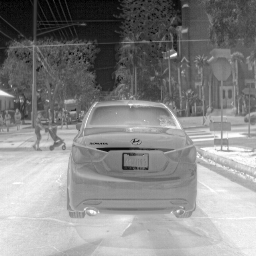
\includegraphics[clip, width=70.32\columnwidth]{images/example/FLIR_10063_real_A.png}}
    \subfigure[可視光]{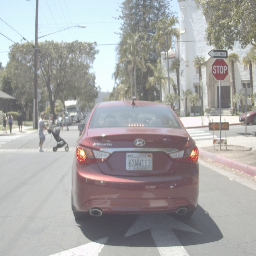
\includegraphics[clip, width=0.32\columnwidth]{images/example/FLIR_10063_real_B.png}}
    \subfigure[既存手法\cite{KUANG_2020_Infrared_TIC-CGAN}]{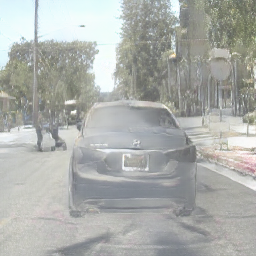
\includegraphics[clip, width=0.32\columnwidth]{images/example/FLIR_10063_fake_B_gll.png}}
    \caption{既存手法による熱赤外線画像の着色}
    \label{fig:tir_to_vis}
\end{figure}

上記の通り,複数のデータセットを用いた実験の結果,提案手法が既存手法と同等かそれ以上の品質で着色が可能であることが定性的・定量的に確認できた.また,複数の被験者によるユーザースタディにおいても提案手法の優位性が示された.さらに,アブレーションスタディを通じて提案するモジュールと損失関数による画像品質の向上が確認された.これは,本論文の提案である,セマンティックセグメンテーションモデルを組み合わせた着色モデルと,クラスに基づく敵対的損失の有効性を示す結果である.



\chapter{関連研究}

\label{chapter:related_work}
\section{白黒画像の着色}
\label{sec:grayscale_colorization}

歴史的価値を持つ画像の視覚的な品質の向上等のために,従来より白黒画像の着色が行われてきた.着色の手法にはユーザーが大まかな色を指定する「走り書き」を用いる手法 \cite{Sykora_2009-LazyBrush} や参照画像を用いる手法 \cite{Gupta_2012_SimilarImage} などが存在するが,近年では深層学習を用いた自動着色手法が活発に研究されており \cite{Iizuka_2016_SIGGRAPH, Su_2020_CVPR_Instance, Zhao_2021_IEEE_SCGAN, Cheng_2015_ICCV_DeepC, Zhao_2018_BMVC_PixellevelSG},ユーザーへの負担の少なさと品質の高さから注目を集めている.\par
%IIZUKA
飯塚ら \cite{Iizuka_2016_SIGGRAPH}は入力画像の大域的な特徴と局所的な特徴の両方を考慮した着色用ネットワークを提案した.これは,中レベル特徴と大域的特徴を別々に抽出し,それらを統合した特徴量から高品質な色度画像を生成可能な着色手法である.\par
%Suら
自動着色で生じやすい物体間での色の混乱を回避するため,Suら \cite{Su_2020_CVPR_Instance} は既存の物体検出器を活用して切り抜いた物体領域だけを着色するインスタンス着色ネットワークと,画像全体に対する着色を行う全画像着色ネットワークを組み合わせたフレームワークを提案し,複数の物体が含まれる画像であっても色滲みを抑えた鮮やかな着色を実現した.\par
%SCGAN
また,Zhaoら \cite{Zhao_2021_IEEE_SCGAN} は重要な領域を表す顕著性マップに基づく注目領域の誘導によって,画像の目立つ部分がより鮮やかで多様な色に着色される視覚的品質の高い手法を提案した.
\par
しかし,これらの手法\cite{Iizuka_2016_SIGGRAPH, Su_2020_CVPR_Instance}は明度画像を入力として色度のみを推定する手法であり,可視光グレースケール画像のように画像の明度成分が既知であることを前提とした手法である.熱赤外線画像の着色においては,画像の色度成分だけではなく可視光画像の明度に対応する成分も推定する必要があり,通常の場合これらの着色手法を適用することはできない.


%2.2
\section{熱赤外線画像の着色}
\ref{sec:grayscale_colorization}節で紹介した通常の白黒画像の着色手法とは別に,熱赤外線画像の着色に特化した手法がいくつか提案されている \cite{Berg_2018_CVPRW_TIR2Lab, KUANG_2020_Infrared_TIC-CGAN, Luo_2022_IEEE_PearlGAN, Liao_2023_IEEE_MUGAN}.\par
%TIR2Lab
Bergら \cite{Berg_2018_CVPRW_TIR2Lab} はエンコーダ・デコーダ構造の畳み込みニューラルネットワーク(CNN)を用いた着色手法を提案した.これは熱赤外線画像からCIELab色空間のLチャネルまたはL,a,b全チャネルを推定する手法で,完全自動の着色が可能であるが,生成される画像はテクスチャを欠く全体的にぼやけたものになっていた.
%TIC-CGAN
これに対し,Kuangら \cite{KUANG_2020_Infrared_TIC-CGAN} は敵対的生成ネットワーク(GAN) \cite{Goodfellow_2014_NIPS_GAN} を用いる手法を提案した.この手法では画像間変換フレームワークであるpix2pix \cite{Isola_2017_CVPR_pix2pix} をベースとしたネットワークを複合的な損失関数を用いて学習させることで,本物らしい詳細なテクスチャを持つ画像を生成することが可能になった.
%MUGAN
最新の研究では,UNet++ \cite{Zhou_2019_IEEE_UNetPlusPlus} で提案された密なスキップ接続とUNet3+ \cite{Huang_2020_ICASSP_UNet3+} で提案されたフルスケールスキップ接続を組み合わせた混合スキップ接続や,デコーダの効果的な情報選択のためのアテンション機構を組み合わせた生成器を着色に使用するGANをLiaoら \cite{Liao_2023_IEEE_MUGAN} が提案し,定性的・定量的に優れた結果を達成した.\par
しかし,いずれの手法においても生成された画像には依然として不自然に着色される領域が存在し,見た目の品質が損なわれている.\par
この問題を解決するため,本論文で提案する手法はセマンティックセグメンテーション用のモデルから有用な特徴量を抽出し,着色モデルが物体の意味情報を生成画像に正しく反映できるよう利用する.

\section{セマンティックセグメンテーション}
セマンティックセグメンテーションとは,与えられた画像の各ピクセルに対して事前に定義されたクラスラベルを割り当てるタスクを指す.このタスクは画像に描写された物体や情景を画素単位で分類,抽象化することができるため,複雑な環境下で周囲の状況を把握する必要がある自動運転や,類似したパターンから所望の領域を発見する必要がある医療用画像分析などにおける利用が注目されている.\par
近年ではCNNが様々な機械学習タスクにおいて高い性能を発揮しており,セマンティックセグメンテーションにおいてもCNN利用の手法が高い精度での自動ラベリングに成功している \cite{Long_2015_CVPR_FCN, Badrinarayanan_2015_ArXiv_SegNet, Ronnenberger_2015_MICCAI_UNet, Chen_2018_ECCV_DeepLabv3plus}.画像のセグメンテーションにCNNを使用した初期の手法の例がFully Convolutional Network(FCN) \cite{Long_2015_CVPR_FCN} である.この手法ではVGG-16 \cite{Simonyan_2015_ICLR_VGG} ネットワークの全結合層を廃して畳み込み層に置換し,End-to-Endで効率的に学習可能なセグメンテーションモデルを実現した.

Ronnebergerらは生医学画像のセグメンテーションのためのCNNとしてU-Net \cite{Ronnenberger_2015_MICCAI_UNet} を提案した.
U-Netは同解像度のレイヤ間を繋ぐスキップ接続によってエンコーダで取得した情報をデコーダに効果的に伝達可能であり,セマンティックセグメンテーションのほか,画像生成などの他タスクにおいても優れた性能を発揮している.本研究の提案手法もU-Netの構造を踏襲した生成器を利用する.\par

また,Googleの研究チームが発表したDeepLabシリーズの最新モデルであるDeepLab v3+ \cite{Chen_2018_ECCV_DeepLabv3plus} も高い性能を示した.DeepLab v3+はDeepLab v3から拡張したエンコーダ・デコーダ構造のセグメンテーション用ネットワークであり,深さ方向への分離可能な畳み込みの適用などによって高速かつ精度の高いセグメンテーションを実現した.




\chapter{提案手法}

\label{sec:proposed_method}

本論文ではセマンティックセグメンテーションモデルを活用し,画像内の各領域が意味的に自然な着色画像を生成可能な手法を提案する.
本章では初めに提案手法の概要を紹介し,続いてセグメンテーションモデルを活用した生成器と学習時の損失関数の詳細について説明する.

\begin{figure*}[tb]
    \centering
    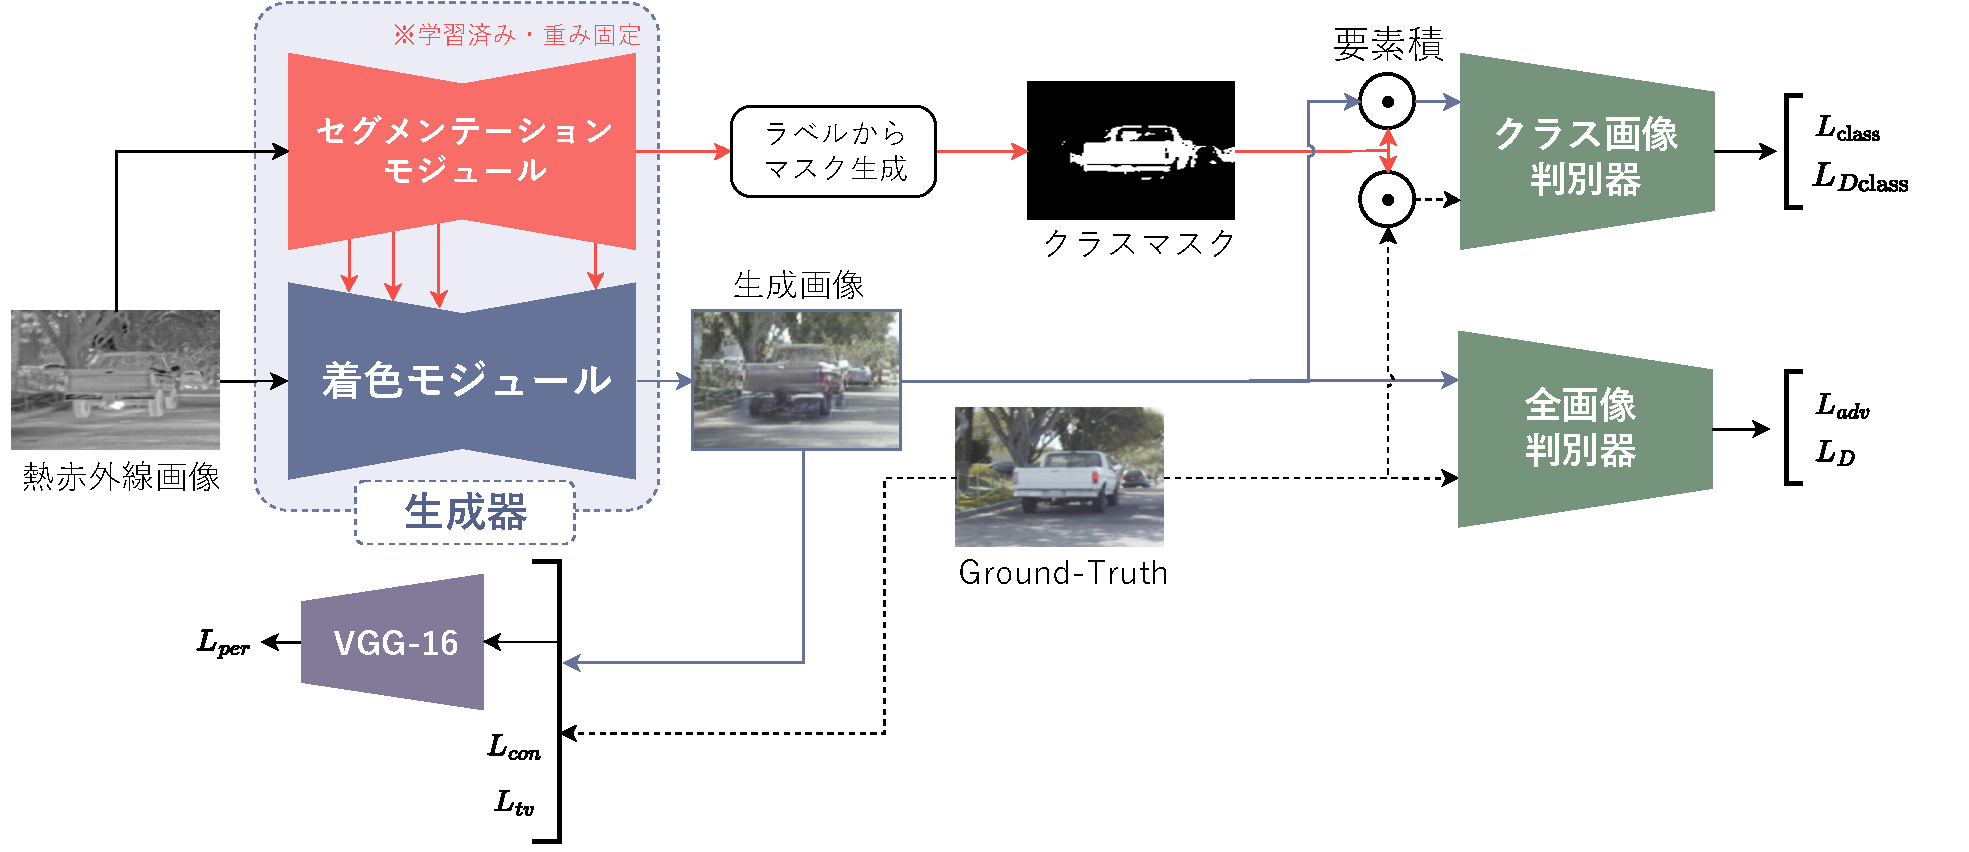
\includegraphics[clip, width=1\columnwidth]{images/overall_architecture-jp_20240114.pdf}
    \caption{提案手法の概要}
    \label{fig:overall_architecture}
\end{figure*}

\begin{figure*}[tb]
    \centering
    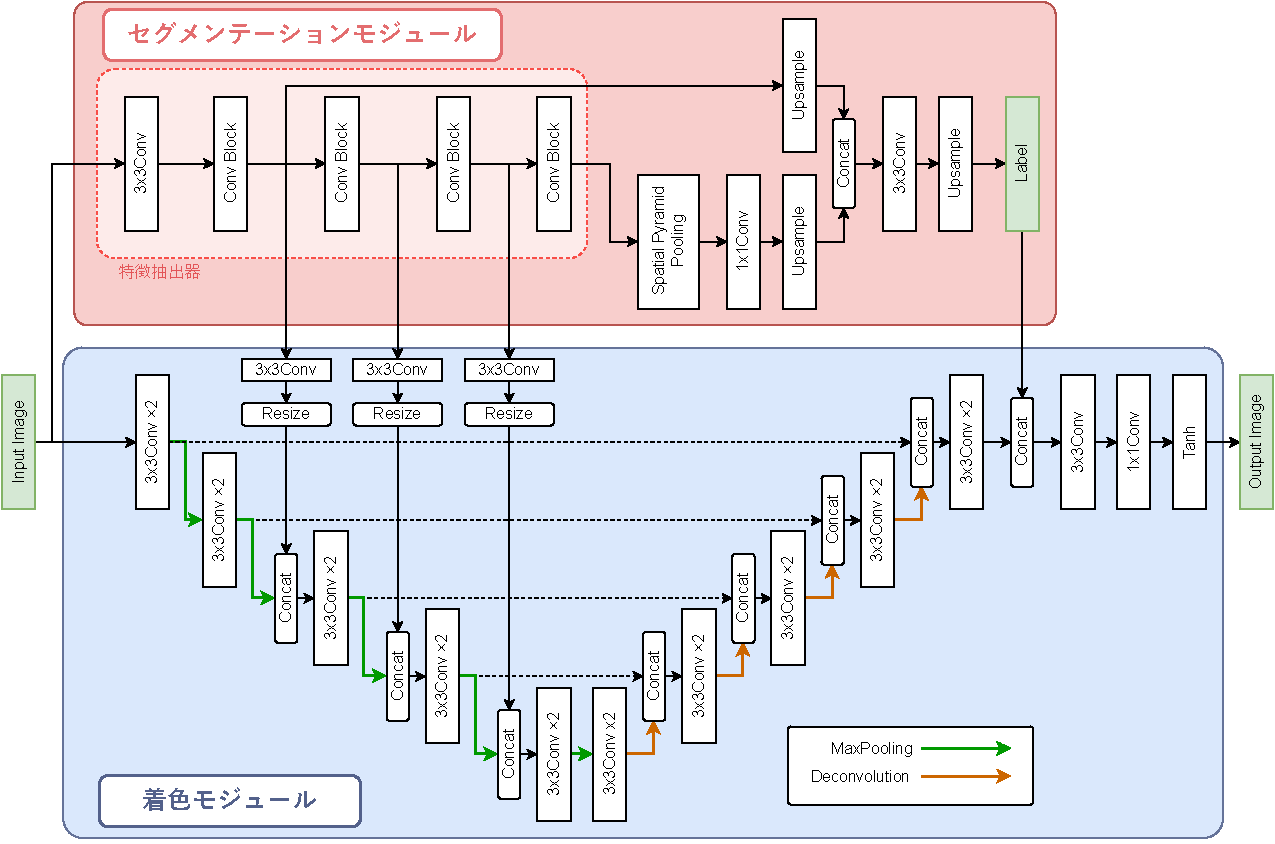
\includegraphics[clip, width=1\columnwidth]{images/generator_architecture-jp_20240114.pdf}
    \caption{生成器の構造}
    \label{fig:generator_architecture}
\end{figure*}

\section{提案手法の概要}
\label{sec:overview}
提案手法の概要を図\ref{fig:overall_architecture} に示す.
図 \ref{fig:overall_architecture}に示す通り,提案手法は着色モジュールとセグメンテーションモジュールから成る生成器,画像全体の真贋判定を行う全画像判別器,特定のクラスに属する領域の真贋判定を行うクラス画像判別器によって構成される敵対的生成ネットワーク \cite{Goodfellow_2014_NIPS_GAN} である.\par
生成器はグレースケールの熱赤外線画像を入力として受け取るネットワークで,セマンティックラベルマップとRGBの着色画像を生成する.生成器を構成するモジュールのうち,着色モジュールは熱赤外線画像をエンコーダ・デコーダ構造のネットワークによりRGBの着色画像へ変換する主モジュールである.
セグメンテーションモジュールは学習済みのセマンティックセグメンテーションモデルであり,着色モジュールへの特徴量の入力とセマンティックラベルの生成を行う.
よく訓練されたセマンティックセグメンテーションモデルは入力画像の各領域と意味ラベルを対応させるのに適した特徴量を抽出しているはずである.
これらの特徴量を,入力画像の各領域の意味を識別するのに有効な情報として与えることで,出力画像の各領域が意味に基づいた適切な色で描画されることが期待できる.
%そのため,セグメンテーションモジュールから抽出した特徴量は入力画像の各領域を意味ごとに区別・分類するのに有効であると考えられ,それを着色モジュールに入力することで,出力画像の各領域がその意味に基づいた色に着色されることが期待できる.
また,セマンティックラベルマップは着色モジュールの補助や後述のクラス敵対的損失の計算のために用いられる.詳細については\ref{subsec:segmentation_module}項,\ref{subsec:colorization_module}項および\ref{subsec:class_adversarial_loss}項に記載している.\par
全画像判別器は着色画像とGround-Truthの全体を受け取るネットワークで,その出力から敵対的損失$L_{adv}$と$L_{D}$の計算を行う.一方でクラス画像判別器はセマンティックラベルマップから作成したクラスマスクを着色画像とGround-Truthそれぞれに適用した画像を受け取るネットワークで,その出力からクラス敵対的損失$L_{class}$と$L_{Dclass}$の計算を行う.クラス敵対的損失は特定のクラス領域のみの画像から計算する敵対的損失であり,詳細な定義については\ref{subsec:class_adversarial_loss}項で述べる.
出力画像全体の真贋判定を行う全画像判別器に加えて,特定のクラス領域の品質に基づいて真贋判定を行うクラス画像判別器を用いることで,生成画像の局所的な品質の向上が期待できる.
なお,両判別器の構造には \cite{Isola_2017_CVPR_pix2pix} で用いられている$70 \times 70$ \ PatchGANを採用する.

\subsection{セグメンテーションモジュール}
\label{subsec:segmentation_module}
セグメンテーションモジュールは図 \ref{fig:generator_architecture} 赤枠部に示される,生成器を構成するモジュールの一つであり,重みを固定した熱赤外線画像用の学習済みセグメンテーションモデルである.
モジュール前段のエンコーダ部の各層は分岐によって着色モジュールのエンコーダ部と接続されており,抽出した特徴量を対応する層に伝達する構造になっている.抽出した特徴量は畳み込みとリサイズによって解像度とチャネル数を調節した後,着色モジュール側の特徴量と結合される.
\ref{sec:overview}節の通り,十分に学習されたセマンティックセグメンテーションモデルは入力画像と「車」や「人物」等の意味ラベルを対応させるのに有効な特徴量を抽出できると考えられる.そのため,このモジュールによって抽出された特徴量を後述の着色モジュールに入力することで,着色モジュールが入力画像の各領域を区別することを助け,領域ごとに適切な色を対応づけられるようになることが期待できる.
一方,モジュール後段のデコーダ部からはセマンティックラベルマップが出力され,着色モジュールの出力直前の畳み込み層に入力される.これは生成の最終プロセスで各画素のラベル情報を与えることで,出力画像のクラス領域毎の着色に一貫性が生まれるよう補正されることを期待したものである.また,セマンティックラベルマップは\ref{subsec:class_adversarial_loss}項のクラス敵対的損失計算時のマスク画像生成にも用いられる.
なお,セグメンテーションモジュールに使用するモデルとしてはDeepLab v3+を選択し,特徴抽出器にはResnet101 \cite{He_2015_CVPR_Resnet} を使用する.\par

\subsection{着色モジュール}
\label{subsec:colorization_module}
着色モジュールは入力の熱赤外線画像から出力の着色画像を生成するモジュールであり,図\ref{fig:generator_architecture}青枠部に示している.このモジュールは前段のエンコーダ部で入力画像の特徴を獲得後,後段のデコーダ部でRGB画像として再構成するエンコーダ・デコーダ構造のネットワークである.コストや技術的な問題から,熱赤外線画像は一般的な可視光画像に比べてエッジやテクスチャなどがぼやけたものになりやすい.そのため,低レベル情報の保持は熱赤外線画像の処理において重要な要素である.そこで着色モジュールではエンコーダ部とデコーダ部の各層を接続するU-Net型のスキップ接続を採用し,浅い層から抽出される低レベル特徴を保持している.

エンコーダ部はセグメンテーションモジュールと接続されており,一部の畳み込み層は前の層の出力とセグメンテーションモジュールから受け取った特徴量の両方をチャネル方向に結合したものを入力として受け取る.エンコーダ部から出力された特徴量はデコーダ部を通じて入力画像と同じ解像度まで復元され,セグメンテーションモジュールから受け取ったセマンティックラベルマップと畳み込みによって融合された後,最終的なRGB画像として出力される.セグメンテーションモジュールから特徴量やセマンティックラベルマップを受け取る理由については\ref{subsec:segmentation_module}項の通り,クラスごとの色の適切な選択や着色の一貫性を期待するためである.なお,エンコーダとデコーダの各層にはアテンション機構としてCoordinate Attention \cite{Hou_2021_CVPR_CAB} を組み込み,特徴マップの位置情報を保持しつつモデルの重要領域への注目を促進している.


\section{目的関数}
Kuangらは \cite{KUANG_2020_Infrared_TIC-CGAN} において,複合的な損失関数で学習することによって着色画像の品質が向上することを実験で示している.本研究ではKuangらの手法における損失関数の組み合わせであるコンテンツ損失,敵対的損失,知覚的損失 \cite{Jhonson_2016_ECCV_PerceptualLosses} ,Total Variation損失 \cite{Aly_2005_IEEE_TotalVariation} に加えて,提案するクラス敵対的損失を組み合わせたものを使用する.

\subsection{コンテンツ損失}
コンテンツ損失$L_{con}$は生成画像全体の色味や質感の傾向を捉えるために課せられる損失であり,入力画像を$x$,Ground-Truthを$y$,生成器の出力を$G( \cdot)$,L1ノルムを$|| \cdot||_{1}$,画像の幅と高さをそれぞれ$W$,$H$としたとき
\begin{flalign}
    \begin{split}
        L_{con} &= \cfrac{1}{WH} \sum_{i=1}^{W} \sum_{j=1}^{H} || y_{i,j}-G(x)_{i,j} ||_{1}
    \end{split}
    \label{eq:loss_content}
\end{flalign}
と表される.\par

\subsection{敵対的損失}
\label{subsec:adversarial_loss}
コンテンツ損失のみを使用した場合,全体が平均的な色で着色された,輪郭がぼやけた出力画像になりやすい.敵対的損失$L_{adv}$を目的関数に追加することで,生成器が詳細なテクスチャを持ったリアルな見た目の画像を出力するように促す.損失の計算方法には \cite{Jolicoeur_2018_arXiv_RelativisticGAN}で提案されているRSGANを用い,全画像判別器$D$の出力を$D( \cdot )$とするとき,生成器のパラメータ更新に用いる$L_{adv}$と全画像判別器のパラメータ更新に用いる$L_{D}$はそれぞれ
\begin{flalign}
        L_{adv} &= -\mathbb{E}_{x,y}[\log{(\text{sigmoid}(D(G(x))-D(y)))}]\\
        L_{D} &= -\mathbb{E}_{x,y}[\log{(\text{sigmoid}(D(y)-D(G(x))))}]
    \label{eq:loss_adv}
\end{flalign}
と表される.$L_{adv}$は全画像判別器がGround-Truthよりも生成画像の方が本物らしいと判断した場合に小さくなるため,生成器がリアルな見た目の画像を生成するように促進する.対して,$L_{D}$は全画像判別器が生成画像よりもGround-Truthの方が本物らしいと判断した場合に小さくなり,全画像判別器が真贋判定を正しく行えるように促進する.\par

\subsection{知覚的損失}
ピクセル単位の比較を行うコンテンツ損失では,Ground-Truthの高レベル特徴を再現することは難しい.そのため,学習済みVGG-16ネットワークを用いて抽出した高レベル特徴に基づく損失を課すことで生成画像がGround-Truthの知覚的な特徴を再現できるように促す.
$\phi_{k}(\cdot)$を学習済みVGG-16の$k$番目層の特徴マップ,$C_k$,$W_k$,$H_k$を特徴マップのチャネル数,幅,高さとするとき,知覚的損失$L_{per}$は
\begin{flalign}
    \begin{split}
        L_{per} &= \sum_{k} \cfrac{1}{C_{k} W_{k} H_{k}} \sum_{i=1}^{W_{k}} \sum_{j=1}^{H_{k}} ||\phi_{k}(y)_{i,j}-\phi_{k}(G(x))_{i,j}||_{1}
    \end{split}
    \label{eq:loss_perceptual}
\end{flalign}
と表される.\par

\subsection{Total Variation損失}
生成画像に生じるノイズを低減し空間的な滑らかさを増強するために,画像の$x$,$y$方向の勾配から計算されるTotal Variation損失を追加する.$\nabla_{x}$を$x$方向の勾配,$\nabla_{y}$を$y$方向の勾配,$|\cdot|$を要素ごとの絶対値とするとき,Total Variation損失$L_{tv}$は
\begin{flalign}
    \begin{split}
        L_{tv} &= \cfrac{1}{WH}\sum|\nabla_{x} G({x})+\nabla_{y} G({x})|\\
    \end{split}
    \label{eq:loss_tv}
\end{flalign}
と表される. \par

\subsection{クラス敵対的損失}
\label{subsec:class_adversarial_loss}
画像全体に対して真贋判定を行う敵対的損失に加えて,同一クラスの領域に対して真贋判定を行い,各クラスに該当する部分の見た目の品質を向上させるための損失としてクラス敵対的損失$L_{class}$を追加する. \par
セグメンテーションモデルの出力クラス数を$C_{class}$,セマンティックラベルマップを$s \in \mathbb{R}^{C_{class} \times H \times W}$,画像の幅方向,高さ方向の画素のインデックスをそれぞれ$i$,$j$,ランダムに選択したクラスを$c$とすると,クラスマスク$M$は
\begin{flalign}
    \begin{split}    
        M_{i,j} =
        \begin{cases}
            1 & (s_{c,i,j}=1)\\
            0 & (s_{c,i,j}=0)
        \end{cases}
    \end{split}
    \label{eq:mask}
\end{flalign}
と表される.
クラス画像判別器の出力を$D_{class}(\cdot)$,要素積の演算子を$\odot$とすると,生成器のパラメータ更新に用いる$L_{class}$とクラス画像判別器のパラメータ更新に用いる$L_{Dclass}$はそれぞれ
\begin{align}
        L_{class} &= -\mathbb{E}_{x,y}[\log{(\text{sigmoid}(D_{class}(M \odot G(x))-D_{class}(M \odot y)))}] \\
        L_{Dclass} &= -\mathbb{E}_{x,y}[\log{(\text{sigmoid}(D_{class}(M\odot  y)-D_{class}(M \odot G(x))))}]
    \label{eq:loss_class}
\end{align}
と表される.\par

\subsection{最終的な目的関数}
以上を踏まえると,最終的な目的関数$L_{all}$は
\begin{flalign}
    \begin{split}
        L_{all} = \lambda_{con} L_{con} + \lambda_{adv} L_{adv} + \lambda_{per} L_{per} + \lambda_{tv} L_{tv} + \lambda_{class} L_{class}
    \end{split}
    \label{eq:loss_all}
\end{flalign}
となる.だたし,$\lambda_{con}$,$\lambda_{adv}$,$\lambda_{per}$,$\lambda_{tv}$および$\lambda_{class}$は損失関数の重みであり,$\lambda_{con}=\lambda_{per}=\lambda_{tv}=1$,$\lambda_{adv}=\lambda_{class}=0.03$である.



\chapter{実験}

%4.1
\section{データセット}
本研究では提案手法の評価のために3つの熱赤外線交通シーンデータセットを使用しており,以下にそれぞれについての詳細を記載した.また,提案手法のセグメンテーションモジュールの学習に用いたデータセットについても記載した.なお\ref{sec:night_experiments}節を除く全ての実験で,昼間に撮影された熱赤外線画像及び可視光カラー画像を使用した.

\subsection{IRVI Traffic}
IRVI Traffic データセット \cite{Li_2021_ACMMM_I2VGAN} (以下,IRVIと呼称)は256$\times$256の解像度の熱赤外線画像と可視光カラー画像のペアデータセットである.学習用に17000枚,昼間テスト用に1000枚の画像を使用した.

\subsection{KAIST Multispectral Pedestrian Detection Benchmark}
KAIST Multispectral Pedestrian Detection Benchmarkデータセット \cite{Hwang_2015_CVPR_KAIST}(以下,KAISTと呼称) は320x256の解像度で撮影された熱赤外線画像と可視光カラー画像のペアデータセットである.データセット全体のうち,学習用に33399枚,昼間テスト用に29178枚,夜間テスト用に15962枚を使用した.

\subsection{FLIR ADAS}
FLIR ADASデータセット \cite{FLIRDataset} (以下,FLIRと呼称)はTeledyne FLIR社が提供している640$\times$512の解像度の熱赤外線画像と可視光カラー画像の公開データセットである.本研究ではデータセット全体のうち \cite{Zhang_2020_ICIP_FLIR-Aligned} によって画素レベルで熱赤外線画像と可視光カラー画像が整列されたものを学習に用いた.学習用に2342枚,昼間テスト用に702枚,夜間テスト用に4535枚を使用した.

\subsection{Cityscapes}
Cityscapesデータセット \cite{Cordts_2016_CVPR_Cityscapes} はセマンティックセグメンテーション用の大規模交通シーンデータセットであり,車載カメラで撮影された可視光カラー画像と画素レベルのセマンティックラベルマップのペアで構成されている.本研究ではこのうち詳細なラベルマップが用意されている2975枚の可視光カラー画像を擬似熱赤外線画像に変換し,セグメンテーションモデルの学習に使用した.

%4.2
\section{実験設定}
データセット中に含まれる画像の枚数より,学習のエポック数はFLIRで100,KAISTとIRVIでは20とした.入力画像のデータ拡張には水平反転とランダムクロップを適用し,モデルへの入力サイズは256x256とした.また,モデルの学習率は0.0002から開始後,エポック数の増加に従って段階的に小さくした.オプティマイザにはAdam \cite{Kingma_2015_ICLR_Adam} を使用し,$\beta_{1}=0.5$,$\beta_{2}=0.999$に設定した.\par
比較する既存手法としては,熱赤外線画像着色の先行研究において比較に用いられることが多いIsolaらのpix2pix \cite{Isola_2017_CVPR_pix2pix},KuangらのTIC-CGAN \cite{KUANG_2020_Infrared_TIC-CGAN},ZhaoらのSCGAN \cite{Zhao_2021_IEEE_SCGAN},及び最新の手法であるLiaoらのMUGAN \cite{Liao_2023_IEEE_MUGAN} を用いた.


\section{評価指標}
評価指標にはPeak Signal-to-Noise Ratio(PSNR),Structural SIMilarity(SSIM),Learned Perceptual Image Patch Similarity(LPIPS) \cite{Zhang_2018_CVPR_LPIPS},Fréchet Inception Distance(FID) \cite{Heusel_2017_NIPS_FID} を選択した.
PSNRとSSIMは値が大きいほど画像の品質が良く,一方でLPIPSとFIDは値が小さいほど画像の品質が良い.
PSNRは画像間の画素単位の輝度差により計算される指標,SSIMは平均や標準偏差などを用いて小領域毎に計算される指標であり,画像から直接計算されるのに対し,LPIPSとFIDは学習済みCNNより得られた特徴量をもとに計算する指標である.また,PSNRとSSIMは画像間の画素単位の復元性と相関が高く,対してLPIPSやFIDは人間の知覚特性と相関が高いとされる.なお,FIDに関してテスト画像が2048枚より少ない場合は,通常よりもネットワークの浅い層を用いて特徴量を抽出し,次元数を2048から減らしたベクトルを用いて計算した.

\begin{table}[tb]
\centering
\caption{昼間熱赤外線画像を着色した際の定量評価結果}
\label{tab:qualitative-result}
\scalebox{1}{%
\begin{tabular}{cc|cccc}
\hline
データセット             & 着色手法   & PSNR  & SSIM  & LPIPS  & FID \\ \hline
\multirow{4}{*}{IRVI}  & pix2pix  & 16.88     & 0.600     & 0.284      & 0.780   \\
                       & TIC-CGAN & 17.96     & 0.664     & 0.221      & \underline{0.395}    \\
                       & SCGAN    & 17.29     & 0.653     & 0.219      & 0.597    \\
                       & MUGAN    & \underline{18.25}     & \underline{0.666}     & \underline{0.204}      & 0.404    \\
                       & 提案手法 & \textbf{18.66}     & \textbf{0.688}     & \textbf{0.198}      & \textbf{0.359}    \\ \hline
\multirow{4}{*}{KAIST} & pix2pix  & 15.68     & 0.471     & 0.399      & 77.38   \\
                       & TIC-CGAN & \underline{16.32}     & \underline{0.546}     & 0.374      & 69.31    \\
                       & SCGAN    & 15.85     & 0.505     & 0.380      & 88.67    \\
                       & MUGAN    & \textbf{16.38}  & \textbf{0.554}    & \underline{0.338}      & \underline{37.44}    \\
                       & 提案手法 & 16.20     & 0.538     & \textbf{0.328}      & \textbf{26.93}    \\ \hline
\multirow{4}{*}{FLIR}  & pix2pix  & 18.25     & 0.583     & 0.299      & \underline{2.414}   \\
                       & TIC-CGAN & 18.73     & 0.601     & 0.276      & 2.703    \\
                       & SCGAN    & 18.43     & 0.614     & 0.301      & 3.847    \\
                       & MUGAN    & \underline{19.60}     & \textbf{0.669}     & \underline{0.243}      & 2.938    \\
                       & 提案手法 & \textbf{19.83}     & \underline{0.662}     & \textbf{0.226}     & \textbf{2.377}    \\ \hline
\end{tabular}%
}
\end{table}

%\section{昼間熱赤外線画像の着色実験}
%はじめに,昼間熱赤外線画像を昼間可視光画像へと変換する実験を行い,既存手法と提案手法の比較を行った.

\section{定量評価}
\label{sec:qualitative_result}
表\ref{tab:qualitative-result}に昼間熱赤外線画像を着色した際の定量評価の結果を示した.
表\ref{tab:qualitative-result}からわかるように,ほぼ全てのデータセットと評価指標の組み合わせで提案手法が最良,またはそれと同等の結果を記録した.特にIRVIにおいては全ての指標で提案手法が最良の結果を示しており,提案手法によって生成された画像がGround-Truthの復元性と知覚的な品質の両方において優位であることがわかった.FLIRにおいても最新の手法であるMUGANと同等か,それを上回る結果であり,比較的小規模なデータセットであっても提案手法は効果的に学習できていると言える.\par
KAISTにおいてはPSNRとSSIMが他手法より僅かに劣っていた.これはKAISTに含まれる熱赤外線画像が比較的低画質・低コントラストであり,セグメンテーションモジュールによる有用な特徴量の獲得が他データセットと比較して困難であったからだと考えられる.一方でLPIPSとFIDにおいては提案手法が最も優れたスコアを示しており,依然として提案手法が高レベルな意味特徴の再現に有効であるということが確認できた.

\begin{figure}[tb]
    \centering
    \includegraphics[clip, width=1\columnwidth]{images/qualitative_result-jp_20240114.pdf}
    \caption{各手法における昼間熱赤外線画像の着色結果}
    \label{fig:qualitative_measure}
\end{figure}

\section{定性評価}
図\ref{fig:qualitative_measure}に各手法における昼間熱赤外線画像の着色結果を示した.なお,上段2行はFLIR,中段2行はKAIST,下段2行はIRVIでの結果である.\par
図\ref{fig:qualitative_measure}の1行目の例からわかるように,pix2pix,TIC-CGAN,SCGANでは前景物体である車両が道路や街路樹と同じ色で着色されており,透けているような見た目となった.MUGANは他の既存手法よりも車両の輪郭が比較的明瞭に現れたが,依然として不自然な出力結果であった.一方で提案手法では車両と道路等の背景がはっきりと異なる色で着色された,比較的自然な見た目の画像が得られた.ブレーキランプやナンバープレートのような細かな色の再現が行われた事も注目すべき点である.
2行目の例では,既存手法のほとんどで中央の人物領域が透けたような見た目になっており,特にSCGANではほぼ完全にシルエットが消失した.一方で提案手法においては黒いシルエット様の着色になっており,人物らしい自然な色合いの再現には至っていないものの,背景領域と明確に区別可能であった.\par
3,4行目のKAISTの例においてもFLIRと同様に,既存手法にて透けているように着色されていた車両部分が,提案手法では車両らしいテクスチャを持つはっきりとした着色になっていることが確認できた.また,既存手法で生じている空の領域のアーティファクトを抑制し,Ground-Truthに近い色で着色できた.\par
5行目の例は提案手法のモデルが画像の意味理解を効果的に行えていたことを示している.既存手法ではトラックの形状とテクスチャを再現することに失敗しており,特にMUGANの例では熱赤外線画像の高輝度領域を道路標識と誤認したことが明らかである.しかし提案手法はトラックに適切な形状とテクスチャを与えることに成功しており,意味的な混乱を回避できていることがわかる.


\section{夜間熱赤外線画像の着色実験}
\label{sec:night_experiments}
熱赤外線カメラは可視光カメラの視界が大きく制限される夜間において優位性を発揮する.したがって,夜間熱赤外線画像の着色は昼間熱赤外線画像の着色よりも実際に利用される可能性が高いシナリオであると考えられる.しかし,同じ熱赤外線画像であっても昼間に撮影した熱赤外線画像と夜間に撮影した熱赤外線画像では輝度分布に異なる特徴が表れる.例えば,日照により物体の温度が平均的に高くなる昼間は画像の輝度値が全体的に近い値になるのに対し,気温が下がる夜間は車両のエンジン部等の強い熱源とその他の部分の輝度差が大きくなる.\par
本節では夜間熱赤外線画像を着色した場合の品質について,提案手法と既存手法を比較し、提案手法の有効性を検証した.評価に用いるデータセットは,夜間熱赤外線画像が含まれるKAIST及びFLIRとした.なお,夜間熱赤外線画像にはペアとなる昼間可視光画像が存在しないため,計算にペアデータが必要なPSNR等の評価指標が使用できない.そのため,定量評価指標には生成画像と参照画像を1対1で対応させる必要が無いFIDのみを用いた.\par
まず,表\ref{tab:night_image_fid}に定量評価結果を示した.表\ref{tab:night_image_fid}から,提案手法が最も優れたFIDスコアを示しており,昼間可視光画像の分布を再現できていることがわかった.
続いて,図\ref{fig:qualitative_night}に各手法における出力結果を示した.なお,1行目がKAIST,2行目がFLIRでの出力結果である.図\ref{fig:qualitative_night}の1行目に示した通り,既存手法では車両が透けているように着色されたり形状に歪みが表れていた一方,提案手法では車両が明瞭で自然な色に着色されたほか,人物のシルエットの視認性が向上していた.また,2行目の例には画像左側の横行する車両の視認性や中央の車両のテクスチャ品質などに提案手法の優位性が表れており,提案手法が全体的に優れた品質の画像を生成できていたことが確認できた.

\begin{table}[tb]
\centering
\caption{夜間熱赤外線画像を着色した際の定量評価結果(FID)}
\label{tab:night_image_fid}
\scalebox{1}{%
\begin{tabular}{l|cc}
\hline
着色手法       & KAIST   & FLIR    \\ \hline
pix2pix      & 168.30  & 90.86    \\
TIC-CGAN     & 108.03  & 74.42    \\
SCGAN        & 142.79  & 80.58    \\
MUGAN        & \underline{93.42}   & \underline{71.88}    \\
提案手法      & \textbf{68.27}   & \textbf{70.15}    \\ \hline
\end{tabular}%
}
\end{table}

\begin{figure}[tb]
    \centering
    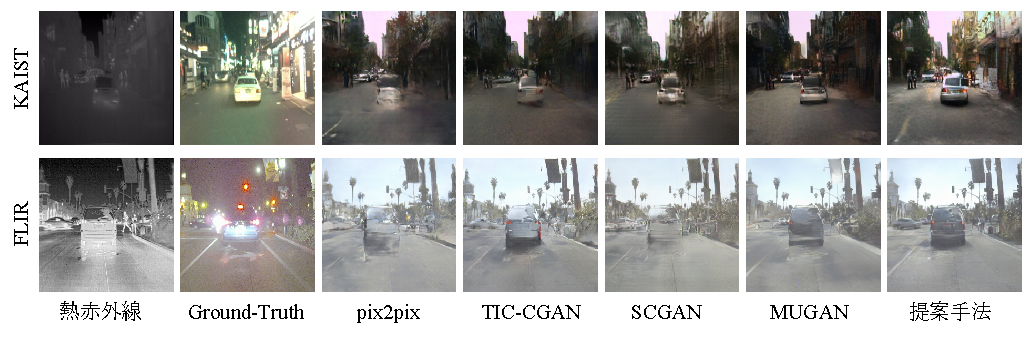
\includegraphics[clip, width=1\columnwidth]{images/qualitative_night-jp_20240114.pdf}
    \caption{各手法における夜間熱赤外線画像の着色結果}
    \label{fig:qualitative_night}
\end{figure}


\section{ユーザースタディ}
\ref{sec:qualitative_result}項では複数の定量評価手法を用いて提案手法の評価を行なったが,それらが必ずしも人間から見た画像の品質と一致するとは限らない.そこで,提案手法と既存手法のどちらの着色画像が優れていると感じるかについて主観評価アンケートを実施することで,提案手法の有効性を評価した.被験者は1問につき提案手法,既存手法及び参照用のGround-Truthの3枚の画像を提示され,画像中の物体をより正しく把握できると感じた画像を2つの手法の中から選択した.実験のデータセットにはKAISTを使用し,比較手法には生成画像の品質が比較的高いMUGAN及びTIC-CGANを選択した.被験者数は19名で,提案手法とMUGANを比較する25問,提案手法とTIC-CGANを比較する25問の計50問に回答した.

\begin{table}[tb]
\centering
\caption{主観評価アンケートの集計結果}
\label{tab:user_study}
\scalebox{1}{
\begin{tabular}{cc|cc|cc}
\hline
\multirow{2}{*}{比較手法} & \multirow{2}{*}{回答数} & \multicolumn{2}{c|}{テスト画像全体} & \multicolumn{2}{c}{有意差がある画像} \\
                          &                  & 枚数[枚]   & 割合[\%]  & 枚数[枚] & 割合[\%] \\ \hline
\multirow{3}{*}{TIC-CGAN} & 「提案手法が良い」が多い     & 25        & 100      & 23       & 100    \\
                          & 「TIC-CGANが良い」が多い    & 0         & 0        & 0        & 0      \\ 
                          & 回答数が等しい     & 0         & 0        & -        & -        \\  \hline
\multirow{3}{*}{MUGAN}    & 「提案手法が良い」が多い     & 19        & 76     & 9        & 90   \\
                          & 「MUGANが良い」が多い       & 6         & 24     & 1        & 10    \\ 
                          & 回答数が等しい     & 0         & 0      & -        & -        \\ \hline
\end{tabular}%
}
\end{table}

表\ref{tab:user_study}中央に,全てのテスト画像に関する集計結果を示した.TIC-CGAN,MUGANともに「提案手法が良い」と回答した割合が「既存手法が良い」と回答した割合を上回った.
また,被験者が「提案手法が良い」または「既存手法が良い」と回答する割合がそれぞれ1/2であるという帰無仮説と,それぞれの割合は異なるという対立仮説を立て,帰無仮説が有意水準5\%で棄却されるか否かによって回答に有意差があるかを判定し,回答に有意差があった画像について集計した結果を表\ref{tab:user_study}右側に示した.これより,有意差がある画像についても「提案手法が良い」と回答した割合の方が大きいという結果が得られた.\par

続いて,図\ref{fig:existing_better}に主観評価アンケートで「既存手法が良い」と回答した割合が高かった画像の例を,図\ref{fig:proposed_better}に「提案手法が良い」と回答した割合が高かった画像の例を示した.

\begin{figure}[tb]
    \centering
    \caption{「既存手法が良い」と回答した割合が高かった画像}
    \label{fig:existing_better}
    \subfigure[熱赤外線]{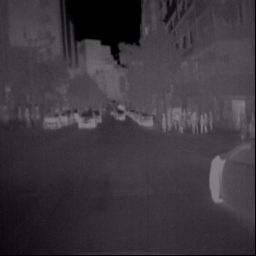
\includegraphics[clip, width=0.24\columnwidth]{images/user_study/existing_better/img24_TIR.png}}
    \subfigure[Ground-Truth]{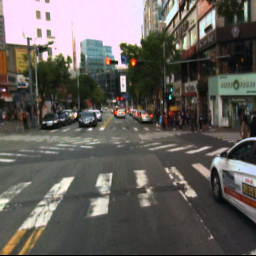
\includegraphics[clip, width=0.24\columnwidth]{images/user_study/existing_better/img24_gt.jpg}}
    \subfigure[既存手法(MUGAN)]{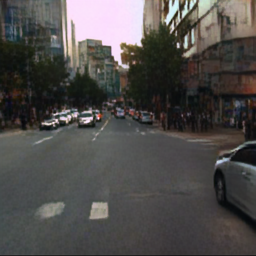
\includegraphics[clip, width=0.24\columnwidth]{images/user_study/existing_better/img24_mu.jpg}}
    \subfigure[提案手法]{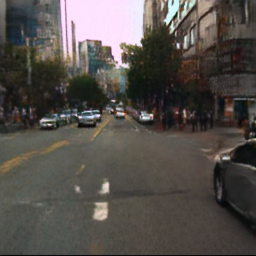
\includegraphics[clip, width=0.24\columnwidth]{images/user_study/existing_better/img24_proposed.jpg}}
\end{figure}

\begin{figure}[tb]
    \centering
    \caption{「提案手法が良い」と回答した割合が高かった画像}
    \label{fig:proposed_better}
    \subfigure[熱赤外線]{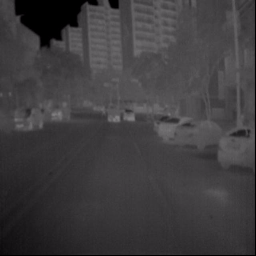
\includegraphics[clip, width=0.24\columnwidth]{images/user_study/proposed_better/img14_TIR.png}}
    \subfigure[Ground-Truth]{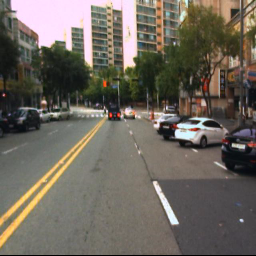
\includegraphics[clip, width=0.24\columnwidth]{images/user_study/proposed_better/img14_gt.jpg}}
    \subfigure[既存手法(MUGAN)]{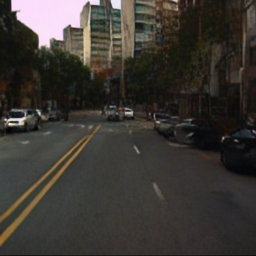
\includegraphics[clip, width=0.24\columnwidth]{images/user_study/proposed_better/img14_mu.jpg}}
    \subfigure[提案手法]{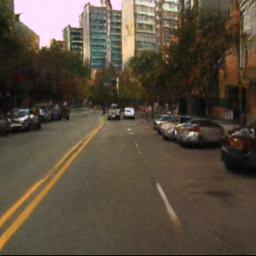
\includegraphics[clip, width=0.24\columnwidth]{images/user_study/proposed_better/img14_proposed.jpg}}
\end{figure}

「既存手法が良い」との回答が多かった画像には,図\ref{fig:existing_better}のように物体の視認性は同程度であるが,提案手法の方が既存手法よりもテクスチャに歪みが見られるものが多く見られた.
一方で「提案手法が良い」との回答が多かった画像は図\ref{fig:proposed_better}のように,既存手法よりも提案手法の方が車両などの前景物体の輪郭がはっきりと確認できるものが多い傾向にあった.以上を踏まえると,提案手法は既存手法において前景物体の視認性が低くなってしまうような入力に対して特に有効であると考えられる.


\section{アブレーションスタディ}
本論文では熱赤外線画像の着色モデルにセグメンテーションモジュールとクラス敵対的損失を利用することを主な提案としている.
本節ではその有効性を検証するため,「セグメンテーションモジュールの有無」と「クラス敵対的損失の有無」に関して条件を変更する実験,およびセグメンテーションモデルから着色モジュールへ入力する特徴量の形式を変更する実験を行った.
なお,実験に使用するデータセットにはIRVIを選択した.\par

\subsection{セグメンテーションモジュールとクラス敵対的損失の効果検証}
\label{subsec:segmentation_and_class_loss}
はじめに,セグメンテーションモジュールとクラス敵対的損失による定量評価スコアの変化を表\ref{tab:ablation_study}に示した.ここで,「Segmentation』はセグメンテーションモジュールの使用に関する項目で,「N/A」は着色モジュールに入力を行わない場合,「Feature」は提案手法と同様にセグメンテーションモジュールで抽出した特徴量を着色モジュールに入力した場合を表している.
表\ref{tab:ablation_study}より,特徴量を入力し,かつクラス敵対的損失を用いている場合(最下段)が全ての指標で最良のスコアを示しており,セグメンテーションモジュールから得た特徴量とクラス敵対的損失の組み合わせが画像の復元性と知覚的品質の両方を向上させていることがわかった.\par
図\ref{fig:ablation_study}にセグメンテーションモジュールの特徴量とクラス敵対的損失による出力画像の変化を示した.ただし,この図には後述の\ref{subsec:feature_type}項における生成結果である「Label\&N/A」および「Label\&$L_{class}$」についても記載している.図\ref{fig:ablation_study}から,クラス敵対的損失を使用したモデルは比較的道路標識の形状や色の乱れが抑えられ,Ground-Truthに近い描写になっていることが確認できた.また,特徴量を入力したモデルは草木が過剰に黒く着色されたり,背後の建造物と同化してしまうような意味的な混乱が抑制されていた.\par


\begin{table}[tb]
\centering
\caption{セグメンテーションモジュールの特徴量と$L_{class}$による定量評価スコアの変化}
\label{tab:ablation_study}
\scalebox{1}{%
\begin{tabular}{cc|cccc}
\hline
Segmentation  & $L_{class}$   & PSNR  & SSIM  & LPIPS  & FID \\ \hline
N/A           & N/A    & \underline{18.56}     & 0.682     & \underline{0.204}      & 0.376    \\
N/A           & \checkmark    & 18.44     & 0.684     & \textbf{0.198}        & 0.363    \\
%Label           & N/A    & \underline{18.56}     & 0.680     & 0.208      & 0.398    \\
%Label           & \checkmark    & 18.53     & \textbf{0.688}          & \underline{0.199}         & 0.382       \\
Feature       & N/A    & 18.48     & \underline{0.685}     & 0.208      & \underline{0.360}    \\
Feature       & \checkmark    & \textbf{18.66} & \textbf{0.688} & \textbf{0.198} & \textbf{0.359}    \\ \hline

\end{tabular}%
}
\end{table}


\begin{figure*}[tb]
    \centering
    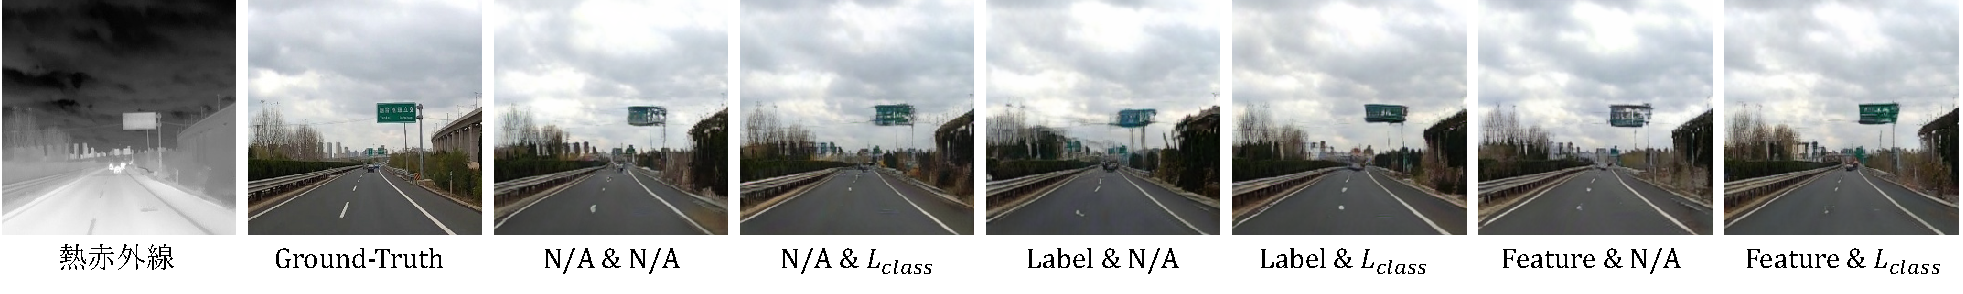
\includegraphics[clip, width=1\columnwidth]{images/ablation_study-jp_20240114.pdf}
    \caption{セグメンテーションモジュールの特徴量と$L_{class}$による出力画像の変化}
    \label{fig:ablation_study}
\end{figure*}


\subsection{着色モジュールへの入力に適した特徴量の検討}
\label{subsec:feature_type}
続いてセグメンテーションモジュールから着色モジュールへの,着色に適した特徴量の入力形式を検討した.比較する特徴量の形式としては,提案手法と同様の「セグメンテーションモジュールの特徴抽出器から抽出した特徴量」と,「セグメンテーションモジュールから出力したセマンティックラベルマップ」の2種類を比較した.\par
表\ref{tab:ablation_study_label}に着色モジュールへ入力する特徴量の形式を変更した際の定量評価の結果を示した.ただし,表中の「Segmentation」の項目が「Label」となっているモデルがセマンティックラベルマップを入力したモデル,「Feature」となっているモデルが特徴抽出器からの特徴量を入力したモデルを表す.表\ref{tab:ablation_study_label}より,特徴抽出器からの特徴量の方がセマンティックラベルマップを入力した場合よりも定量評価が良くなる傾向が見られた.また前述の通り,図\ref{fig:ablation_study}にはセマンティックラベルマップを入力したモデルの出力画像も記載したが,\ref{subsec:segmentation_and_class_loss}項の結果と同様に,草木などの着色において特徴抽出器からの特徴量を用いたモデルに優位性が見られた.これは,クラス情報のみを保持するセマンティックラベルマップそのものよりも,特徴抽出器からの特徴量の方が着色に有効な情報を豊富に保持しているためだと考えられる,

\begin{table}[tb]
\centering
\caption{着色モジュールへ入力する特徴量の形式による定量評価スコアの変化}
\label{tab:ablation_study_label}
\scalebox{1}{%
\begin{tabular}{cc|cccc}
\hline
Segmentation  & $L_{class}$   & PSNR  & SSIM  & LPIPS  & FID \\ \hline
%N/A           & N/A    & \underline{18.56}     & 0.682     & {0.204}      & 0.376    \\
%N/A           & \checkmark    & 18.44     & 0.684     & \textbf{0.198}        & 0.363    \\
Label           & N/A    & \underline{18.56}     & 0.680     & 0.208      & 0.398    \\
Label           & \checkmark    & 18.53     & \textbf{0.688}          & \underline{0.199}         & 0.382       \\
Feature       & N/A    & 18.48     & \underline{0.685}     & 0.208      & \underline{0.360}    \\
Feature       & \checkmark    & \textbf{18.66} & \textbf{0.688} & \textbf{0.198} & \textbf{0.359}    \\ \hline
\end{tabular}%
}
\end{table}



\section{クラス敵対的損失の重みの検討}
クラス敵対的損失の最適な重みの値について調査するため,IRVIデータセットを用いて実験を行った.表\ref{tab:loss_weight}にクラス敵対的損失の重みを変化させた際の定量評価スコアの変化を示した.表\ref{tab:loss_weight}からからわかるように,$\lambda_{class}=0.03$が他に比べてバランスが良く優れたスコアを示していた,したがってクラス敵対的損失の重みとしては$\lambda_{class}=0.03$が適切であると考えられる.

\begin{table}[tb]
\centering
\caption{クラス敵対的損失の重みによる定量評価スコアの変化}
\label{tab:loss_weight}
\scalebox{1}{%
\begin{tabular}{c|cccc}
\hline
損失の重み   & PSNR & SSIM  & LPIPS  & FID \\ \hline
$\lambda_{class} = 0$ & \underline{18.48}     & \underline{0.685}     & 0.208      & {0.360}    \\
$\lambda_{class} = 0.003$ & {18.36}     & {0.681}     & \underline{0.202}      & \textbf{0.353}    \\
$\lambda_{class} = 0.03$  &  \textbf{18.66}     & \textbf{0.688}     & \textbf{0.198}  & 0.359 \\
$\lambda_{class} = 0.3$   & 18.12     & 0.680     & 0.207      & \underline{0.357}    \\
$\lambda_{class} = 3$     & \underline{18.48}     & \underline{0.685}     & 0.206      & \underline{0.357}       \\ \hline
\end{tabular}%
}
\end{table}


\section{敵対的損失の種類の変更}
本節では提案手法の学習時に適用する敵対的損失の計算方法を変更した際の結果を比較し,提案手法に適したGANの種類について調査した. 比較するGANの種類は提案手法で使用しているRSGAN\cite{Jolicoeur_2018_arXiv_RelativisticGAN},通常のGAN(Vanilla \ GAN)\cite{Goodfellow_2014_NIPS_GAN}およびLSGAN \cite{Mao_2016_CVPR_LSGAN}とし,表 \ref{tab:GAN_type}にその定量評価結果を示した.\par

\begin{table}[tb]
\centering
\caption{敵対的損失の計算方法による定量評価スコアの変化}
\label{tab:GAN_type}
\scalebox{1}{%
\begin{tabular}{c|cccc}
\hline
GAN の種類         & PSNR            & SSIM           & LPIPS          & FID             \\ \hline
Vanilla          & \underline{18.24}         & \textbf{0.699} & \underline{0.204}        & 0.390           \\
LSGAN            & \underline{18.24}           & 0.685          & 0.210          & \underline{0.384}           \\
%WGAN-GP         & a               & b              & c              & d               \\
RSGAN(提案手法で使用)  & \textbf{18.66}  & \underline{0.688}          & \textbf{0.198} & \textbf{0.359}  \\ \hline
\end{tabular}%
}
\end{table}

表 \ref{tab:GAN_type} に示したとおり,RSGANがほぼ全ての指標で最も優れた結果を記録した.
RSGANは判別器の真贋判定が生成画像の品質のみに注目することを回避するため,生成画像とGroun-Truth間の相対的な本物らしさを損失として用いている.これによりGround-Truthの情報を通常のGAN等よりも効果的に活用できるとされており,この特性がRSGAN使用時の生成画像の品質を向上させたのだと考えられる.


\section{学習データとテストデータに関する検討}
学習データが与える出力画像への影響を調査するため,学習データとテストデータの組み合わせを変更する実験を行った.この実験ではKAIST,FLIR,IRVIのいずれかのデータセットで学習したモデルに対し,全てのデータセットのテスト画像を入力した.\par

\begin{figure}[tb]
    \centering
    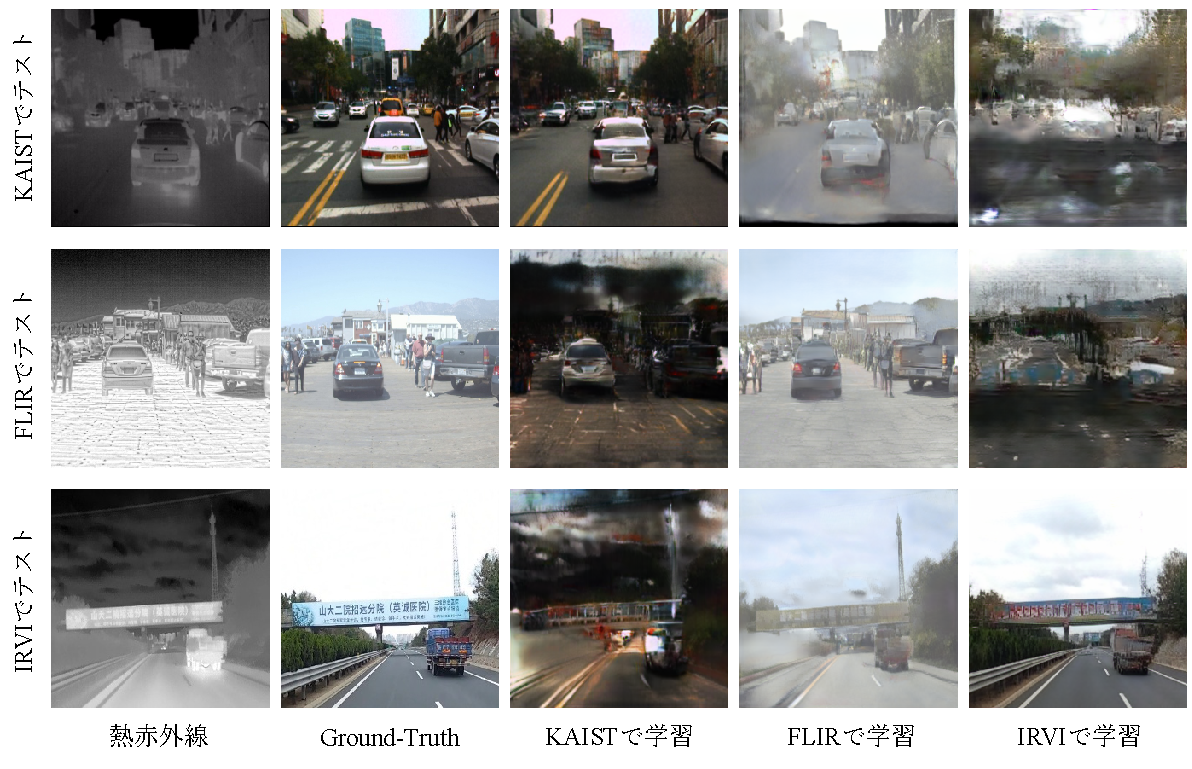
\includegraphics[clip, width=1\columnwidth]{images/dataset_swap-jp_20240114.pdf}
    \caption{学習データセットとテストデータセットの組み合わせを変更した際の着色画像の変化}
    \label{fig:dataset_swap}
\end{figure}

図\ref{fig:dataset_swap}にデータセットの組み合わせを変更した際の着色画像の変化を示した.図\ref{fig:dataset_swap}からわかる通り,学習データセットとテストデータセットが異なると生成画像の品質が著しく悪化した.これについて最も大きな原因は,各データセットで使用している熱赤外線カメラの違いが考えられる.
例えば,KAISTは解像度$320\times256$のFLIR A35カメラで撮影されているのに対し,FLIRはより解像度の高い$640\times512$のFLIR Tau2カメラで撮影されている.また,ゲインの自動制御やディティール強調など,撮影時に適用される画像処理もデータセットごとに異なる.そのため,取得される熱赤外線画像の特徴がデータセットごとに異なり,着色モデルがその違いに適応しきれずに品質が悪化したのだと考えられる.\par
また,他の原因としてはデータセットに含まれるシーンのバリエーションの違いが挙げられる.学習に使用したデータセットは交通シーンであることは共通しているものの,各データセットが内包するシーンの種類や数はそれぞれ異なる.例えば,KAISTやFLIRが比較的多様なシーンを含むのに対してIRVIは単一のシーンのみを含むデータセットであるが,学習の際にIRVIのような多様なシーンを含まないデータセットを使用するとモデルの表現力が低くなり,異なるデータセットに適応できなくなると考えられる.\par

学習データとテストデータの違いによる失敗例が確認された一方で,学習とテストでデータセットが同じ場合であっても一部のテスト画像では自然な着色に失敗した.図\ref{fig:failure_case}はその例である.図\ref{fig:failure_case}上段の例では,トンネル内の風景を自然に着色することに失敗していることがわかる.学習データセット内に類似したシーンがほとんど存在しないデータが入力された場合,この例の様に自然な色を再現できず乱れた着色結果が生成されてしまう.また,図\ref{fig:failure_case}下段の例では木のテクスチャを再現することに失敗して過剰に暗く描写されているほか,芝がアスファルトのように着色されている.この例は入力画像にテクスチャやエッジの表現に十分な輝度差が無い領域が存在し,可視光画像の再現に必要な特徴を満足に得られなかったことが原因であると考えられる.以上の様な着色の失敗は,より多様な状況下で撮影された高品質なデータを学習に利用することや,入力画像に対してコントラスト強調などの処理を加えることで回避できる可能性がある.

\begin{figure}[tb]
    \centering
    \caption{学習データセットとテストデータセットが同じだが適切に着色できなかった例}
    \label{fig:failure_case}
    \subfigure{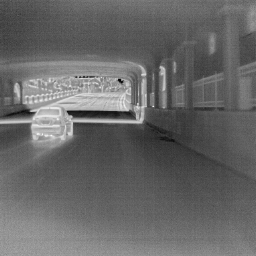
\includegraphics[clip, width=0.32\columnwidth]{images/failure/FLIR_09243_real_A.png}}
    \subfigure{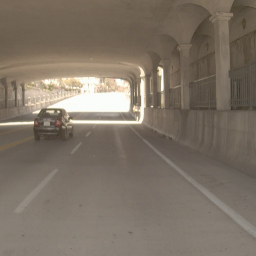
\includegraphics[clip, width=0.32\columnwidth]{images/failure/FLIR_09243_real_B.png}}
    \subfigure{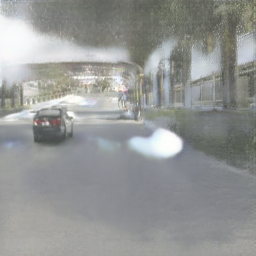
\includegraphics[clip, width=0.32\columnwidth]{images/failure/FLIR_09243_fake_B.png}} \\
    \subfigure[熱赤外線]{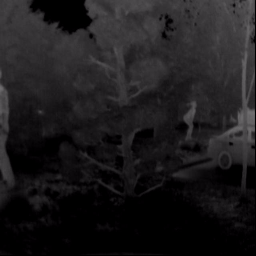
\includegraphics[clip, width=0.32\columnwidth]{images/failure/set06_V004_I00132_real_A.png}}
    \subfigure[Ground-Truth]{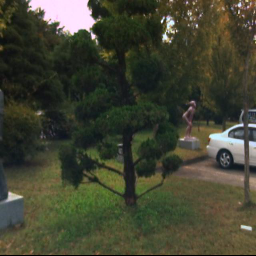
\includegraphics[clip, width=0.32\columnwidth]{images/failure/set06_V004_I00132_real_B.png}}
    \subfigure[着色画像]{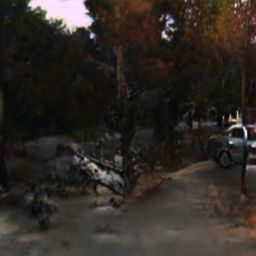
\includegraphics[clip, width=0.32\columnwidth]{images/failure/set06_V004_I00132_fake_B.png}}
\end{figure}




\chapter{結論}

本論文では意味情報を考慮して熱赤外線画像から高品質な着色画像を生成する手法を提案した.提案手法は学習済みセマンティックセグメンテーションモデルを利用して熱赤外線画像から有用な特徴を獲得し,着色モデルに入力することでモデルの意味理解を強化する.また,特定クラスに属する領域の画像に対する判別器を追加することで局所的な品質を向上する.実験の結果,提案手法は複数のデータセットで既存手法と同等,またはそれを上回る品質の画像を生成できることが確認できた.さらに,アブレーション研究を通じて本手法で提案するセグメンテーションモジュールとクラス敵対的損失が着色の品質向上に有効であることが示された.今後の課題は更なる画像の高品質化に加え,モデルの計算コストの削減などにより高速に学習可能な手法を実現することである.




\bibliographystyle{plain} % 参考文献
\bibliography{myref} %
\chapter*{謝辞}
\addcontentsline{toc}{chapter}{謝辞}

本研究を進めるにあたり,多大なるご指導を頂いたとともに,研究の機会を与えてくださった東北大学大学院工学研究科 大町真一郎教授に心より感謝申し上げます.

本研究をまとめるにあたり,審査委員として貴重なご意見をいただきました,東北大学電気通信研究所 本間尚文教授,東北大学電気通信研究所 塩入諭教授に心より感謝申し上げます.

本研究を進めるにあたり,私の相談に親身に乗っていただき,様々なご指導やご助言をいただきました,東北大学大学院工学研究科 宮崎智助教に心より感謝申し上げます.

また,日ごろより議論,助言,楽しい研究室生活をいただいた同期,および先輩方や後輩方に心より感謝申し上げます.

最後に,学生生活の機会をいただき支えとなってくださった家族,勉学や研究を共に励んだ友人に感謝の意を表します.
\chapter*{研究業績}
\addcontentsline{toc}{chapter}{研究業績}

{\bf 学会発表} \\

\noindent ``物体のテクスチャに注目したGANによる熱赤外線画像着色手法の検討''\\
\noindent 宇川慧,宮崎智,大町真一郎,\\
\noindent 第 25 回 画像の認識・理解シンポジウム (MIRU2022)\\
\noindent インラタクティブセッション,IS3-52(2022-07)\\
%\appendix
\chapter{その他の実験}
\section{夜間TIR画像に対する着色}
TIRカメラは可視光カメラの視界が大きく制限される夜間において優位性を発揮する.したがって,夜間TIR画像の着色は昼間TIR画像の着色よりも実際に利用される可能性が高いシナリオであると考えられる.しかし,同じTIR画像であっても昼間に撮影したTIR画像と夜間に撮影したTIR画像では輝度分布に異なる特徴が表れる.例えば,日照により物体の温度が平均的に高くなる昼間は画像の輝度値が全体的に近い値になるのに対し,気温が下がる夜間は車両のエンジン部等の熱源とその他の部分の輝度差が大きくなる.
本節では夜間TIR画像を各手法を用いて着色し,昼間の可視光画像に変換した際の品質を比較することで,提案手法の夜間TIR画像に対する有効性を検証する.評価に用いるデータセットは夜間TIR画像が含まれるKAIST及びFLIRデータセットとし,テスト画像の枚数はKAISTが15962枚,FLIRが4535枚とする.また,定量評価指標にはFIDを用いる.\par
まず,表\ref{tab:night_image_fid}に定量評価結果を示す.表\ref{tab:night_image_fid}から,提案手法が最も優れたFIDスコアを示しており,昼間可視光画像の分布を再現できていることがわかる.
続いて,図\ref{fig:qualitative_night}に各手法における出力結果を示す.なお,1行目がKAISTデータセット,2行目がFLIRデータセットでの出力結果である.図\ref{fig:qualitative_night}の1行目からは,既存手法では車両が透けているように着色されたり形状に歪みが表れている一方,提案手法では車両が明瞭で自然な色に着色されているほか,人物のシルエットの視認性が向上していることがわかる.また2行目では,画像左側の横行する車両の視認性や中央の車両のテクスチャ品質などから提案手法の優位性が確認でき,全体的に優れた品質の画像を生成できていることがわかる.

\begin{table}[tb]
\centering
\caption{夜間TIR画像を着色した場合の定量評価(FID)}
\label{tab:night_image_fid}
\scalebox{1}{%
\begin{tabular}{l|cc}
\hline
着色手法       & KAIST   & FLIR     \\ \hline
pix2pix      & 168.30  & 90.86    \\
TIC-CGAN     & 108.03  & 74.41    \\
SCGAN        & 142.79  & 80.58    \\
MUGAN        & \underline{93.42}   & \underline{71.88}    \\
提案手法      & \textbf{67.06}   & \textbf{70.15}    \\ \hline
\end{tabular}%
}
\end{table}

\begin{figure}[tb]
    \centering
    \includegraphics[clip, width=1\columnwidth]{images/qualitative_night_jp.pdf}
    \caption{各手法における夜間TIR画像の着色結果}
    \label{fig:qualitative_night}
\end{figure}

\section{ユーザースタディ}
本研究では複数の定量評価手法を用いて提案手法の評価を行なっているが,それらが必ずしも人間から見た画像の品質と一致するとは限らない.そこで,提案手法と既存手法のどちらの着色画像が優れていると感じるかについて主観評価アンケートを実施することで,提案手法の有効性を評価する.被験者は提案手法,既存手法及び参照用のGround-Truthの3枚の画像を一度に提示され,画像中の物体をより正しく把握できると感じた画像を2つの手法の中から選択する.実験にはKAISTデータセットを使用し,比較手法は生成画像の品質が比較的高いMUGAN及びTIC-CGANとする.被験者数は18名で,提案手法とMUGANを比較する25問,提案手法とTIC-CGANを比較する25問の計50問に回答する.
表\ref{tab:user_study}に主観評価アンケートの結果を示す.

\begin{table}[tb]
\centering
\caption{主観評価アンケートの集計結果}
\label{tab:user_study}
\scalebox{1}{
\begin{tabular}{cc|cc|cc}
\hline
\multirow{2}{*}{比較手法} & \multirow{2}{*}{回答数} & \multicolumn{2}{c|}{テスト画像全体} & \multicolumn{2}{c}{有意差がある画像} \\
                          &                  & 枚数[枚]   & 割合[\%]  & 枚数[枚] & 割合[\%] \\ \hline
\multirow{3}{*}{TIC-CGAN} & 「提案手法が良い」が多い     & 25        & 100      & 23       & 100    \\
                          & 「TIC-CGANが良い」が多い    & 0         & 0        & 0        & 0      \\ 
                          & 回答数が等しい     & 0         & 0        & -        & -        \\  \hline
\multirow{3}{*}{MUGAN}    & 「提案手法が良い」が多い     & 18        & 72     & 9        & 90   \\
                          & 「MUGANが良い」が多い       & 5         & 20     & 1        & 10    \\ 
                          & 回答数が等しい     & 2         & 8      & -        & -        \\ \hline
\end{tabular}%
}
\end{table}

表\ref{tab:user_study}中央は,全てのテスト画像に関する集計結果である.ここからTIC-CGAN,MUGANともに「提案手法が良い」と回答した割合が「既存手法が良い」と回答した割合を上回っていることがわかる.
また,被験者が「提案手法が良い」または「既存手法が良い」と回答する割合がそれぞれ1/2であるという帰無仮説と,それぞれの割合は異なるという対立仮説を立て,帰無仮説が有意水準5\%で棄却されるか否かによって回答に有意差があるかを判定し,回答に有意差があった画像について集計した結果が表\ref{tab:user_study}右側である.これより,有意差がある画像についても「提案手法が良い」と回答した割合の方が大きいことがわかる.\par

続いて,図\ref{fig:existing_better}に主観評価アンケートで「既存手法が良い」と回答した割合が高かった画像の例を,図\ref{fig:proposed_better}に「提案手法が良い」と回答した割合が高かった画像の例を示す.

\begin{figure}[tb]
    \centering
    \caption{「既存手法が良い」と回答した割合が高かった画像}
    \label{fig:existing_better}
    \subfigure[TIR]{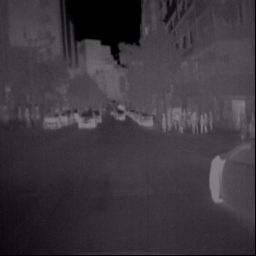
\includegraphics[clip, width=0.24\columnwidth]{images/user_study/existing_better/img24_TIR.png}}
    \subfigure[Ground-Truth]{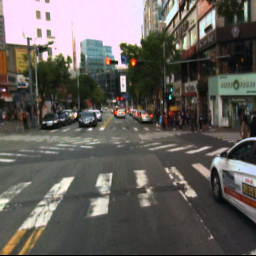
\includegraphics[clip, width=0.24\columnwidth]{images/user_study/existing_better/img24_gt.jpg}}
    \subfigure[提案手法]{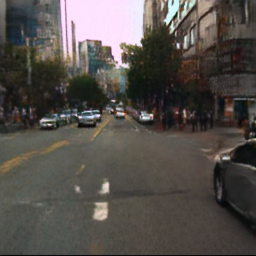
\includegraphics[clip, width=0.24\columnwidth]{images/user_study/existing_better/img24_proposed.jpg}}
    \subfigure[既存手法(MUGAN)]{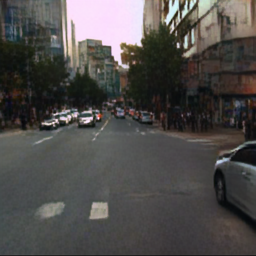
\includegraphics[clip, width=0.24\columnwidth]{images/user_study/existing_better/img24_mu.jpg}}
\end{figure}

\begin{figure}[tb]
    \centering
    \caption{「提案手法が良い」と回答した割合が高かった画像}
    \label{fig:proposed_better}
    \subfigure[TIR]{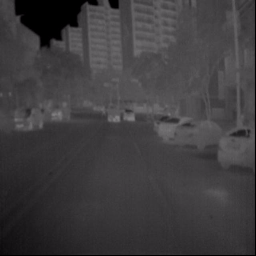
\includegraphics[clip, width=0.24\columnwidth]{images/user_study/proposed_better/img14_TIR.png}}
    \subfigure[Ground-Truth]{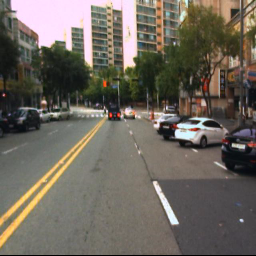
\includegraphics[clip, width=0.24\columnwidth]{images/user_study/proposed_better/img14_gt.jpg}}
    \subfigure[提案手法]{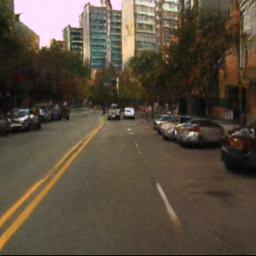
\includegraphics[clip, width=0.24\columnwidth]{images/user_study/proposed_better/img14_proposed.jpg}}
    \subfigure[既存手法(MUGAN)]{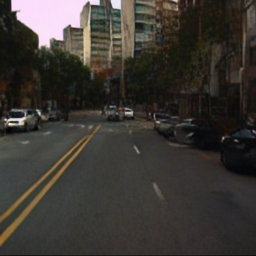
\includegraphics[clip, width=0.24\columnwidth]{images/user_study/proposed_better/img14_mu.jpg}}
\end{figure}

「既存手法が良い」との回答が多かった画像には,図\ref{fig:existing_better}のように物体の視認性は同程度であるが,提案手法の方が既存手法よりもテクスチャに歪みが見られるものが多く見られた.
一方で「提案手法が良い」との回答が多かった画像は図\ref{fig:proposed_better}のように,既存手法よりも提案手法の方が車両などの前景物体の輪郭がはっきりと確認できるものが多い傾向にあった.以上を踏まえると,提案手法は既存手法において前景物体の視認性が低くなってしまうような入力に対して特に有効であると考えられる.

\section{学習データとテストデータの組み合わせの変更}
本節では学習データが与える出力画像への影響を調査するため,学習データとテストデータの組み合わせを変更して着色画像の生成を行う.学習に用いたデータセットのテスト画像に加え,学習に用いなかったデータセットのテスト画像をモデルに入力すること.\par
図\ref{fig:dataset_swap}にデータセットの組み合わせを変更した際の着色画像の変化を示す.

\begin{figure}[tb]
    \centering
    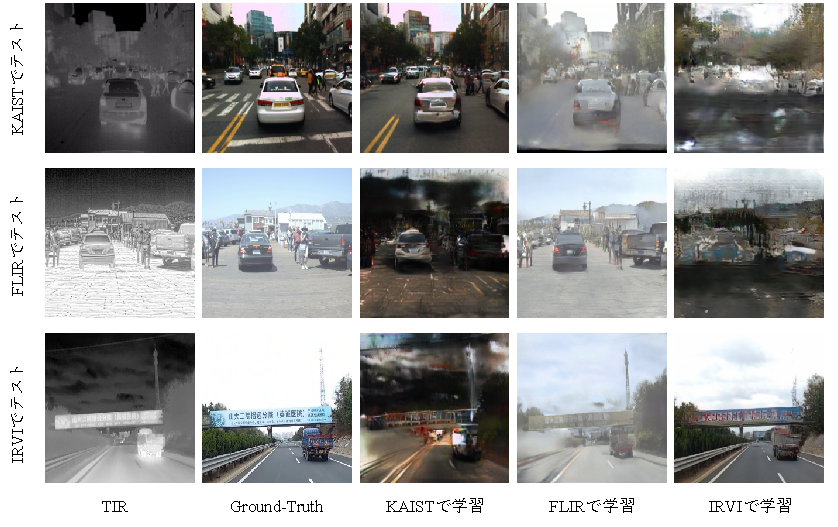
\includegraphics[clip, width=1\columnwidth]{images/dataset_swap.pdf}
    \caption{学習データセットとテストデータセットの組み合わせを変更した際の着色画像の変化}
    \label{fig:dataset_swap}
\end{figure}

図\ref{fig:dataset_swap}から,学習データセットとテストデータセットが異なると生成画像の品質が著しく悪化することがわかる.考えられる品質悪化の原因の一つとして,データセット間の輝度分布の違いが挙げられる.
例えば,FLIRやIRVIは全体的に高コントラストであるため空の領域に比較的輝度が高い領域が存在する一方で,KAISTは全体的に低輝度・低コントラストであるため空の領域の輝度はほとんど0になっている.そのため,KAISTで学習したモデルに他のデータセットの画像を入力すると輝度差によりモデルが混乱し,空の領域を黒く塗りつぶすような不適切な着色が行われたと考えられる.\par
また,他の原因としてはデータセットに含まれるシーンのバリエーションの違いが挙げられる.
図\ref{fig:dataset_swap}では特にIRVIデータセットで学習したモデルの出力画像に大きな歪みが認められるが,KAISTやFLIRが比較的多様なシーンを含むデータセットであるのに対してIRVIが単一のシーンのみを含むデータセットであり,汎化性能が低くなったためだと考えられる.
\end{document}






